\section{Proposta}
A grande motivação para o desenvolvimento deste balanceador de carga proveio do desígnio da melhoria e correção de alguns problemas de um BC que utilizando uma abordagem gulosa na composição de seu algoritmo, onde trabalhava com a idéia de calcular a média aritmética do processador e com base nesse calculo então decidir qual tarefa iria ser migrada de fato. O Almejo de um ganho maior de desempenho na realização de testes com grandes cargas computacionais, dimanou na criação de um novo balanceador de carga que também utiliza uma abordagam centralizada, com uma estratégia de tomada de decisão um pouco diferente. Culminando em um ganho significativo de desempenho em relação a este BC específico e também a outros balanceadores que utilizam diferentes estratégias de tomada de decisão. O balanceador de carga em questão levou o nome de \newlb.    


\section{Metodologias de Implementação}

Atualmente muitas aplicações são dinâmicas ou realizam grandes cálculos computacionais, demandando cada vez de mais capacidade computacional. De acordo com \cite{padoin2014saving}, o grande problema por trás disso é que na maioria das vezes não há uma preocupação com o desbalanceamento de carga gerado por estas aplicações, impedindo que as máquinas paralelas aproveitem todo o seu potencial. Na figura \ref{img_load_balance_unbalance} podemos notar a diferença entre um processador balanceado e um que não está balanceado.

\begin{figure}[!htb]
	\centering
	\caption{Diferença Entre um Processador com Carga Desbalanceada e Balanceada}
	\centering
	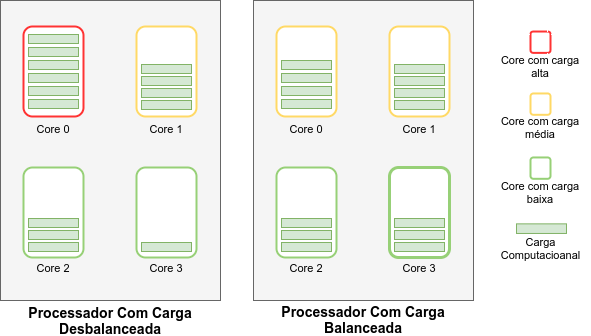
\includegraphics[scale=0.50]{figuras/load_balance.png}
	\label{img_load_balance_unbalance}
	\centering
\end{figure}

Também baseado nesse problema é que o \newlb foi desenvolvido buscando atingir o estado de equilíbrio entre os processadores rapidamente, sem partir diretamente para os chares mais carregados evitando migrações desnecessárias. O BC proposto possui uma abordagem centralizada, então o processo de tomada de decisão e a estrutura de cargas e comunicação da máquina ficam armazenadas em um único computador. Em virtude de realizar um balanceamento de carga mais preciso e trabalhar muito bem com escalabilidade é que foi escolhido a abordagem centralizada.

Durante o processo de execução, o BC coleta dados dos processadores e da aplicação
e os armazena em um banco de dados de balanceamento de cargas. Dentre estas informações,
destacam-se o número total de objetos, a carga total de cada processador, a carga de cada
objeto e o número total de processadores.Estes dados serão utilizados na hora de decidir quais chares devem ser migrados e qual valor cada processador deve ter para estar em equilíbrio.

O \newlb foi desenvolvido utilizando o framework de balanceamento de cargas disponibilizado pelo \charm. Este framework de balanceamento de carga foi escolhido uma vez que permite tanto a criação de um novo BC quanto a utilização dos BCs disponibilizados pelo ambiente para comparações de resultados.

O \charm adota uma metodologia baseada na medição das cargas das tarefas que executam em cada core. Para isso, o framework coleta automaticamente estatísticas da carga computacional e da comunicação destes objetos e armazena tais informações em uma base de dados que pode ser utilizada pelos BC para a tomada de decisões \cite{jyothi2004debugging}.


\section{Algoritmo}

Na Figura \ref{img_smartlb_effect} é exemplificado o funcionamento da estratégia de tomada de decisão do \newlb. A partir de informações fornecidas pelo \charm, o algoritmo proposto busca atingir ba lanceamento levando em consideração a diferença de carga entre o core mais carregado e o menos carregado. Desta forma, migra tarefas do core mais carregado para o core com menor carga, buscando equilibrar a carga total do sistema, reduzir o número de migrações e reduzir o tempo total de execução da aplicação.

\begin{figure}[!htb]
	\centering
	\caption{Balanceamento de carga executado pelo \newlb}
	\centering
	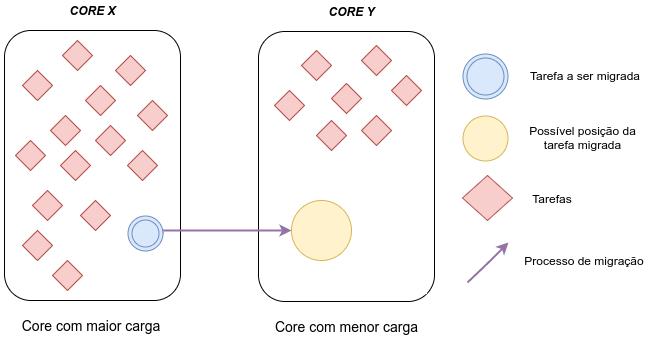
\includegraphics[scale=0.40]{figuras/smartlb_load_balance.png}
	\label{img_smartlb_effect}
	\centering
\end{figure}

A estratégia utilizada para implementação do balanceamento de carga proposto constitui-se de melhorias nas estrategias utilizadas nos algoritmos \greedylb e \refinelb. Nossas melhorias buscam equilibrar as cargas entre os processadores reduzindo o número de migrações, adotando um threshold para definir o desbalanceamento de carga aceitável.

Na Tabela 1 são apresentados os principais parâmetros utilizados na implementação do
algoritmo proposto.

\begin{table}[h]
	\centering
	\caption{Principais parâmetros utilizados no algoritmo \newlb}
	\vspace{0.5cm}
	\resizebox{.6\columnwidth}{!}{
		\label{tab:parametros}
		\begin{tabular}{l|l}
			\hline
			\textbf{Parâmetro} & \textbf{Definição} \\
			\hline
			$ PM $ & Core com maior carga \\
			$ Pm $ & Core com menor carga \\ 
			
			$ D $ & Desbalanceamento entre $PM$ e $Pm$ \\
			
			$ ct $ & Carga da tarefa $P$ \\
			$ nTarefas $ &  Número de tarefas\\
			
			$ getCoreAtual(i) $ & Retorna o processador atual da tarefa\\
			$ getCargaTarefa()     $ & Retorna a carga da tarefa\\
			$ getCargaMaior() 	     $ & Retorna a carga do core mais carregado \\
			$ getCargaMenor()        $ & Retorna a carga do core menos carregado \\
			
			$ migrarProcesso(i, PM, Pm) $ & Migrar tarefa $i$ de $ PM $ para $ Pm $ \\
			
			
			\hline
		\end{tabular}
} \end{table}


Quando o balanceador é aplicado primeira mente verifica as cargas do core mais carregado e o core menos carregado, a partir dessa informação ele analisa a diferença de carga entre o core mais e menos carregado. Caso essa diferença for maior que o \textit{threshold} definido o balanceador busca tarefas do processador mais carregado testando se a carga da tarefa é menor ou igual ao desbalanceamento. Caso seja, ele realiza a migração desta tarefa do core mais carregado para o menos carregado e encontra o novo core mais carregado e o novo processador menos carregado, como demonstrado no Algoritmo 1. 

\begin{table}[h]
	\centering
	%\caption{Algoritmo: \avg}
	%\vspace{0.5cm}
	\resizebox{.4\columnwidth}{!}{
		\label{tab:algoritmo}
		\begin{tabular}{cl}
			%  \hline
			\multicolumn{2}{c}{Algoritmo 1: Implementação do \newlb} \\
			\hline
			& $~~~$\\
			
			1 & $PM = getCargaMaior();$  \\
			2 & $Pm = getCargaMenor();$  \\
			3 & $\textbf{if}( (Pm / PM ) > Threshold)$ \{ \\
			4 & $~~~~~~~\textbf{for}(i=1; i<=nTarefas; i++)$ \{ \\
			5 & $~~~~~~~~~~~~\textbf{if}(getCoreAtual(i) == PM)$ \{ \\
			6 & $~~~~~~~~~~~~~~~~ ct = getCargaTarefa(i);$  \\
			7 & $~~~~~~~~~~~~~~~~ D = PM-Pm;$  \\
			8 & $~~~~~~~~~~~~~~~~~ \textbf{if}(ct <= D)$ \{\\
			9 & $~~~~~~~~~~~~~~~~~~~~~~migrarProcesso(i, PM, Pm);$ \\
			10 & $~~~~~~~~~~~~~~~~~~~~~\textbf~ PM = getCargaMaior(); $\\
			11 & $~~~~~~~~~~~~~~~~~~~~~\textbf~ Pm = getCargaMenor(); $\\
			12 & $~~~~~~~~~~~~~~~~~ \}$ \\
			13 & $~~~~~~~~~~~~ \}$ \\
			14 & $~~~~~~ \}$ \\
			15 & $\} $\\
			%     \hline
		\end{tabular}
	}
\end{table} 

Desta forma, consegue-se um balanceamento de carga mais preciso, pois caso o desbalanceamento entre o core mais e menos carregado muito pequeno o algoritmo não irá realizar nenhuma ação, e quando esse desbalanceamento for grande ele migra somente tarefas que carga menor a diferença. evitando muitas migrações desnecessárias. Após a execução, quando não existem mais cores a serem mapeados e as cargas de todas as unidades de processamento possuem um valor próximo um do outro, o balanceamento é encerrado. 
